\documentclass{article}
\usepackage[T1]{fontenc}
\usepackage{lmodern}
\usepackage{graphicx}
\usepackage{amsmath,amssymb}
\usepackage[a4paper,margin=2cm]{geometry}
\usepackage[absolute,overlay]{textpos}
\setlength{\TPHorizModule}{1mm}
\setlength{\TPVertModule}{1mm}
\usepackage[indonesian]{babel}
\usepackage{hyperref}
\setlength{\emergencystretch}{2em}
% unit: Halaman 38

\begin{document}

% === Halaman 38 (python/native) ===

How Wiretapping Works

(sumber: http://www.howstuffworks.com/wiretapping.htm)

38

When you open up a phone, you can see that the 

technology inside is very simple. The simplicity 

of design makes the phone system vulnerable to 

surreptitious eavesdropping.

Inside a standard phone cord, you'll find a red 

wire and a green wire. These wires form a circuit 

like the one you might find in a flashlight. Just 

as in a flashlight, there is a negatively-charged 

end and a positively-charged end to the circuit. 

In a telephone cord, the green wire connects to 

the positive end and the red cord connects to 

the negative end.

% deskripsi: gambar native xref 237
\noindent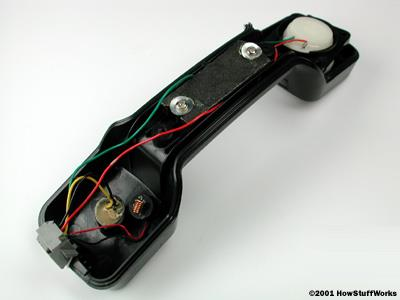
\includegraphics[width=0.85\textwidth]{../../images/python/page_038_img_01.jpeg}

% deskripsi: gambar native xref 238
\noindent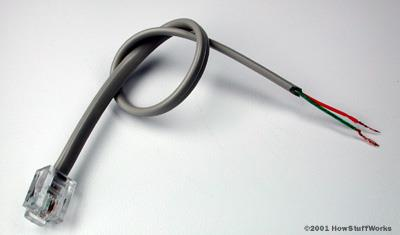
\includegraphics[width=0.85\textwidth]{../../images/python/page_038_img_02.jpeg}

\end{document}
